\section{Second Part (Non-Rigid structure from motion by non-linear optimization and assuming a low-rank shape model)}
\noindent In this task we should perform a nonlinear optimization for a non-rigid body, assuming a low rank. This code uses Levenberg-Marquardt algorithm to optimize the non-linear equation that it is shown to next:
\begin{equation}\label{eq:optimization}
	\underset{R^{i},B_{k},l_{i}^{k},t^{i}}{\arg\min}
	\sum_{i=1}^{i}\Vert \widehat{W}^{i}-R^{i}\sum_{k=1}^{k}l_{i}^{k}B_{k}-t^{i}\Vert^{2}+
	\gamma\sum_{i=1}^{i-1}\Vert L^{i}-L^{i+1} \Vert^{2}+
	\phi\sum_{i=1}^{i-1}\Vert R^{i}-R^{i+1} \Vert^{2}
\end{equation}
\noindent Where:
$B_{k}$ is a row of bases matrix.
$R^{i}$ is a rotation for a point in matrix column $i$ of $X$, which is the 3D shape vector. 
$l_{i}$ are the constants such that $\sum_{k=1}^{k}l_{i}^{k}B_{k}=X$.
$t^{i}$ is the translation.
$L^{i}$ is the vector of all constants in frame $i$.
\noindent The norm used is the Frobenius norm.\\

\noindent In order to calculate the Levenberg-Marquardt optimization, we need to calculate the Jacobian form of the equation \ref{eq:optimization}. We do this as shown in the following slide Figure \ref{fig:slideT2}

\begin{figure}[h]
	\centering
	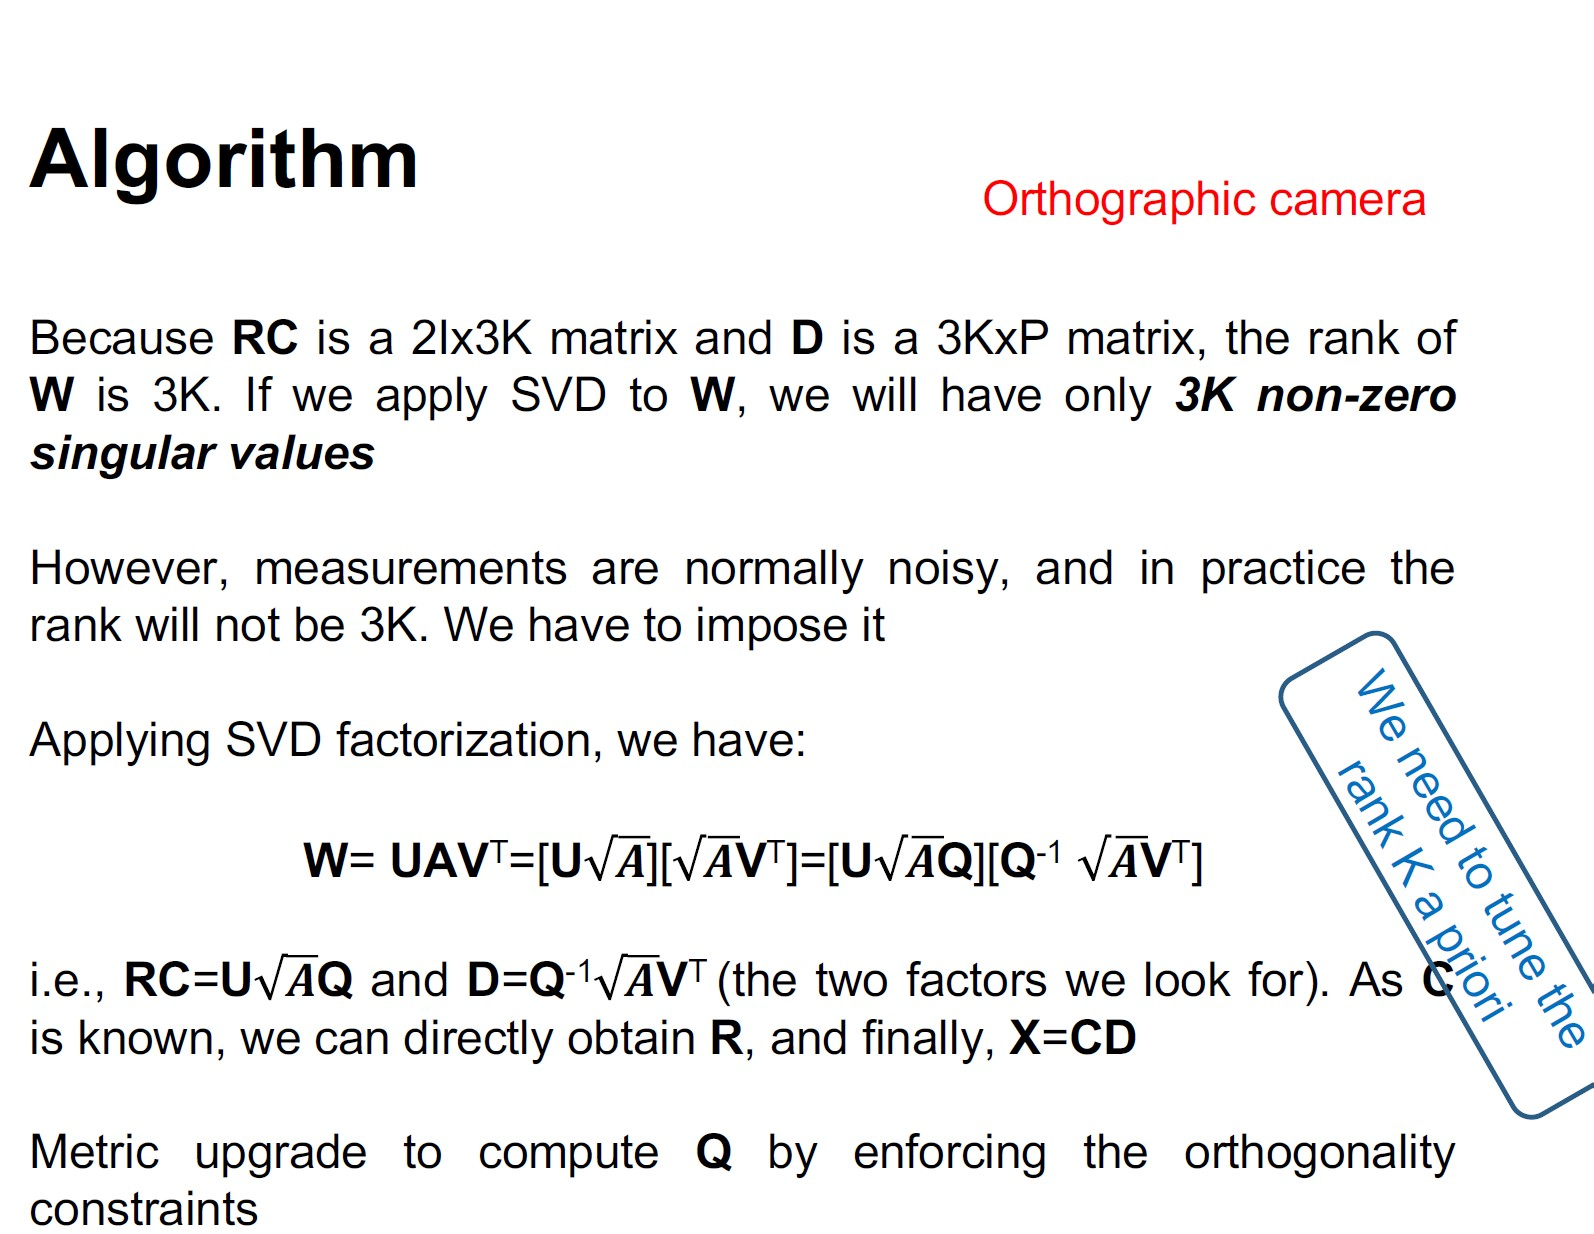
\includegraphics[width=0.7\textwidth]{T2/slide}
	\caption{Jacobian form}
	\label{fig:slideT2}
\end{figure}

\subsection{Code:}
\noindent Now we will show how this Jacobian form is calculated in the code.\\

\noindent So first we will define the dimensions of Jacobian matrix. For this code we are using quaternions for the rotations, therefore $R^{i}$ is $2\times 4$.\\

\noindent Then the dimension of Jacobian matrix is defined in the following way

\begin{itemize}
	\item number of rows of $Dim(J^{rows})=$
	\textcolor{green}{$2\sum_{i=1}^{f}(number of points visible in frame i)$}
	\item number of columns of $Dim(J_{columns})=$
	\textcolor{red}{$4f$}$+$
	\textcolor{blue}{$2f$}$+$
	\textcolor{orange}{$kf$}$+$
	\textcolor{Yellow}{$3kp$}	
\end{itemize}

\noindent Where $f$ is the number of frames, $p$ is the total number of points tracked and $k$ is the total number of bases.\\

\noindent \textbf{Explaining row sizes:}\\
\noindent \textbf{\textcolor{green}{Green}:} Represents the visible points per frame. When we multiply the sum of the visible points by two it is because the rotations are in quaternions. The quaternions are 2x4 and then they are two vectors per each point and that is why it is multiplied by two.\\ 

\noindent \textbf{Explaining column sizes:}\\

\noindent \textbf{\textcolor{red}{Red}:} Represents the value of the columns of the rotation matrix, which is $2\times 4$ quaternions. We have a rotation matrix $R^{i}$ for each frame $i$. Therefore, the dimension is $4f$, where $f$ is the number of frames.\\ 

\noindent \textbf{\textcolor{blue}{Blue}:} Represents the translation matrix $t^{i}$, whose dimension is $1\times 2$, for each frame $i$. Therefore, the dimension is $2f$, where $f$ is the number of frames.\\

\noindent \textbf{\textcolor{orange}{Orange}:} Represents the matrix $L_{i}$, whose dimension is $1\times k$ for each frame $i$. Therefore, the dimension is $kf$, where $f$ is the number of frames.\\

\noindent \textbf{\textcolor{yellow}{Yellow}:} Represents the matrix $B_{b}$, whose dimension is $3\times p$ for each base $b$. Therefore, the dimension is $3pk$, where $k$ is the number of bases.\\

\noindent Well, then we need to define the shape of our Jacobian matrix by putting $1$ where there are values and leaving $0$ in the spaces that do not exist, as shown in the following code.\\

\begin{lstlisting}[style=Matlab-editor, numbers=left]
for i=1:n_frames
        for j=1:nnz(vij(i,:))        
            J(2*j-1+computed_points:2*j+computed_points,6*j-5:6*j)=ones(2,6);
            J(2*j-1+computed_points:2*j+computed_points,K*j-K+1+6*n_frames:K*j+6*n_frames)=ones(2,K);
            J(2*j-1+computed_points:2*j+computed_points,3*K*j-3*K+1+(6+K)*n_frames:3*K*j+(6+K)*n_frames)=ones(2,3*K);
        end
        computed_points=computed_points+2*nnz(vij(i,:));
    end
\end{lstlisting}
\noindent In the first for loop each frame is iterated, in the second for loop only the points visible in that frame are iterated.\\
\begin{lstlisting}[style=Matlab-editor]
J(2*j-1+computed_points:2*j+computed_points,6*j-5:6*j)=ones(2,6);
\end{lstlisting}
\noindent Here, the Jacobian is calculated for the rotation part $R$, in quaternions, and the translation part $t$, having this
\begin{equation}
\begin{pmatrix}
R_{2\times 4} & | & t_{2\times 2}
\end{pmatrix}_{2\times 6}
\end{equation}
we can add a matrix of ones of $2\times 6$

\noindent Now, the Jacobian is calculated for the constants part $L^{i}$, where $L^{i}=[l_{1}^{i},l_{2}^{i}, \cdots, l_{k}^{i}]$ such that $i$ is a frame.
\begin{lstlisting}[style=Matlab-editor]
J(2*j-1+computed_points:2*j+computed_points,K*j-K+1+6*n_frames:K*j+6*n_frames)=ones(2,K);
\end{lstlisting}
and for that, in the code is added a matrix of ones from $2\times k$.\\

\noindent Then, the Jacobian is calculated for the bases part $B_{i}$, where
\begin{equation}
B_{i}=\begin{pmatrix}
[b_{1}^{i}]_{3\times 1} & [b_{2}^{i}]_{3\times 1} & \cdots & [b_{k}^{i}]_{3\times 1}
\end{pmatrix}_{3\times k}
\end{equation}
\begin{lstlisting}[style=Matlab-editor]
J(2*j-1+computed_points:2*j+computed_points,3*K*j-3*K+1+(6+K)*n_frames:3*K*j+(6+K)*n_frames)=ones(2,3*K);
\end{lstlisting}
\noindent and for that, in the code is added a matrix of ones from $2\times 3k$.\\ 

\noindent So, we calculate the Jacobian part of the priors.\\
\begin{equation}\label{eq:priors}
\underset{R^{i},B_{k},l_{i}^{k},t^{i}}{\arg\min}
\gamma\sum_{i=1}^{i-1}\Vert L^{i}-L^{i+1} \Vert^{2}+
\phi\sum_{i=1}^{i-1}\Vert R^{i}-R^{i+1} \Vert^{2}
\end{equation}
\noindent from the equation we have

\begin{itemize}
\item \textbf{The prior with respect to the rotation $R^{i}$:} This means that the rotation between two consecutive frames $\sum_{i=1}^{i-1}\Vert L^{i}-L^{i+1} \Vert^{2}$ do not have abrupt changes, it is a smoothing of the rotations. 
\item \textbf{The prior with respect to the constants $L^{i}$:} This means that the constants, which multiply the bases, such that $X^{i}=\sum_{j=1}^{k}l^{i}_{j}B_{j}$ form the shape matrix. Therefore, if the constants for two consecutive frames $\sum_{i=1}^{i-1}\Vert L^{i}-L^{i+1} \Vert^{2}$ do not have abrupt changes, then the shapes do not have abrupt changes, and for this reason, it is a smoothing of the shapes.
\end{itemize}

\noindent We use the expressions in equation \ref{eq:priors} to calculate the dimension of the Jacobian for the priors.\\

\noindent So from the equation \ref{eq:priors} and the orange color of the Explaining column sizes for the Jacobian matrix, we deduce that the Jacobian dimension for the prior L would be 

\begin{equation}
Dim(J_{rows})=f-1
Dim(J_{columns})=kf
\end{equation}
\noindent and the blue and red color of the Explaining column sizes for the Jacobian matrix, we can deduce the Jacobian dimension for the prior $R$ as 
\begin{equation}
Dim(J_{rows})=f-1
Dim(J_{columns})=6f
\end{equation}

\noindent Now we will show how we fill the indices that have a value in the Jacobian Matrix of the $L$ prior with 1 and otherwise hold with zero.\\
\begin{lstlisting}[style=Matlab-editor]
if (priors.coeff_prior == 1)
     % prior terms on L
     L=spalloc(n_frames-1,(K+6)*n_frames + K*3*n_points,2*K*(n_frames-1));     
     for i=1:n_frames-1
        L(i,K*i-K+1+6*n_frames:K*i+K+6*n_frames)=ones(1,2*K);        
     end
     if K==1
         J(2*nnz(vij)+1:size(J,1), :)=L;
     else
         J(2*nnz(vij)+1:2*nnz(vij)+n_frames-1, :)=L;
     end
 end 
\end{lstlisting}
\noindent We do the following, we take the $L_{i}$ and $L_{i+1}$ and join them as shown in the equation \ref{eq:Li_li1}
\begin{equation}\label{eq:Li_li1}
\begin{pmatrix}
[L_{i}]_{1\times k} & | & [L_{i+1}]_{1\times k}
\end{pmatrix}_{1\times 2k}
\end{equation}
\noindent obtaining a merged matrix with dimensions $1\times 2K$, whose elements are all ones.\\

\noindent For the Jacobian Matrix of the $R$ prior is the similar way, in this case we joint $R^{i}$ and $R^{i+1}$ like show in the equation \ref{eq:Ri_Ri1}
\begin{equation}\label{eq:Ri_Ri1}
\begin{pmatrix}
[R^{i}]_{1\times 6} & | & [R_{i+1}]_{1\times 6}
\end{pmatrix}_{1\times 12}
\end{equation}
\noindent obtaining a merged matrix with dimensions $1\times 12$, whose elements are all ones.\\
\noindent Joining the Jacobian and the two Jacobians of the priors we have the following graph figure \ref{fig:J}. 

\begin{figure}[h]
    \centering
    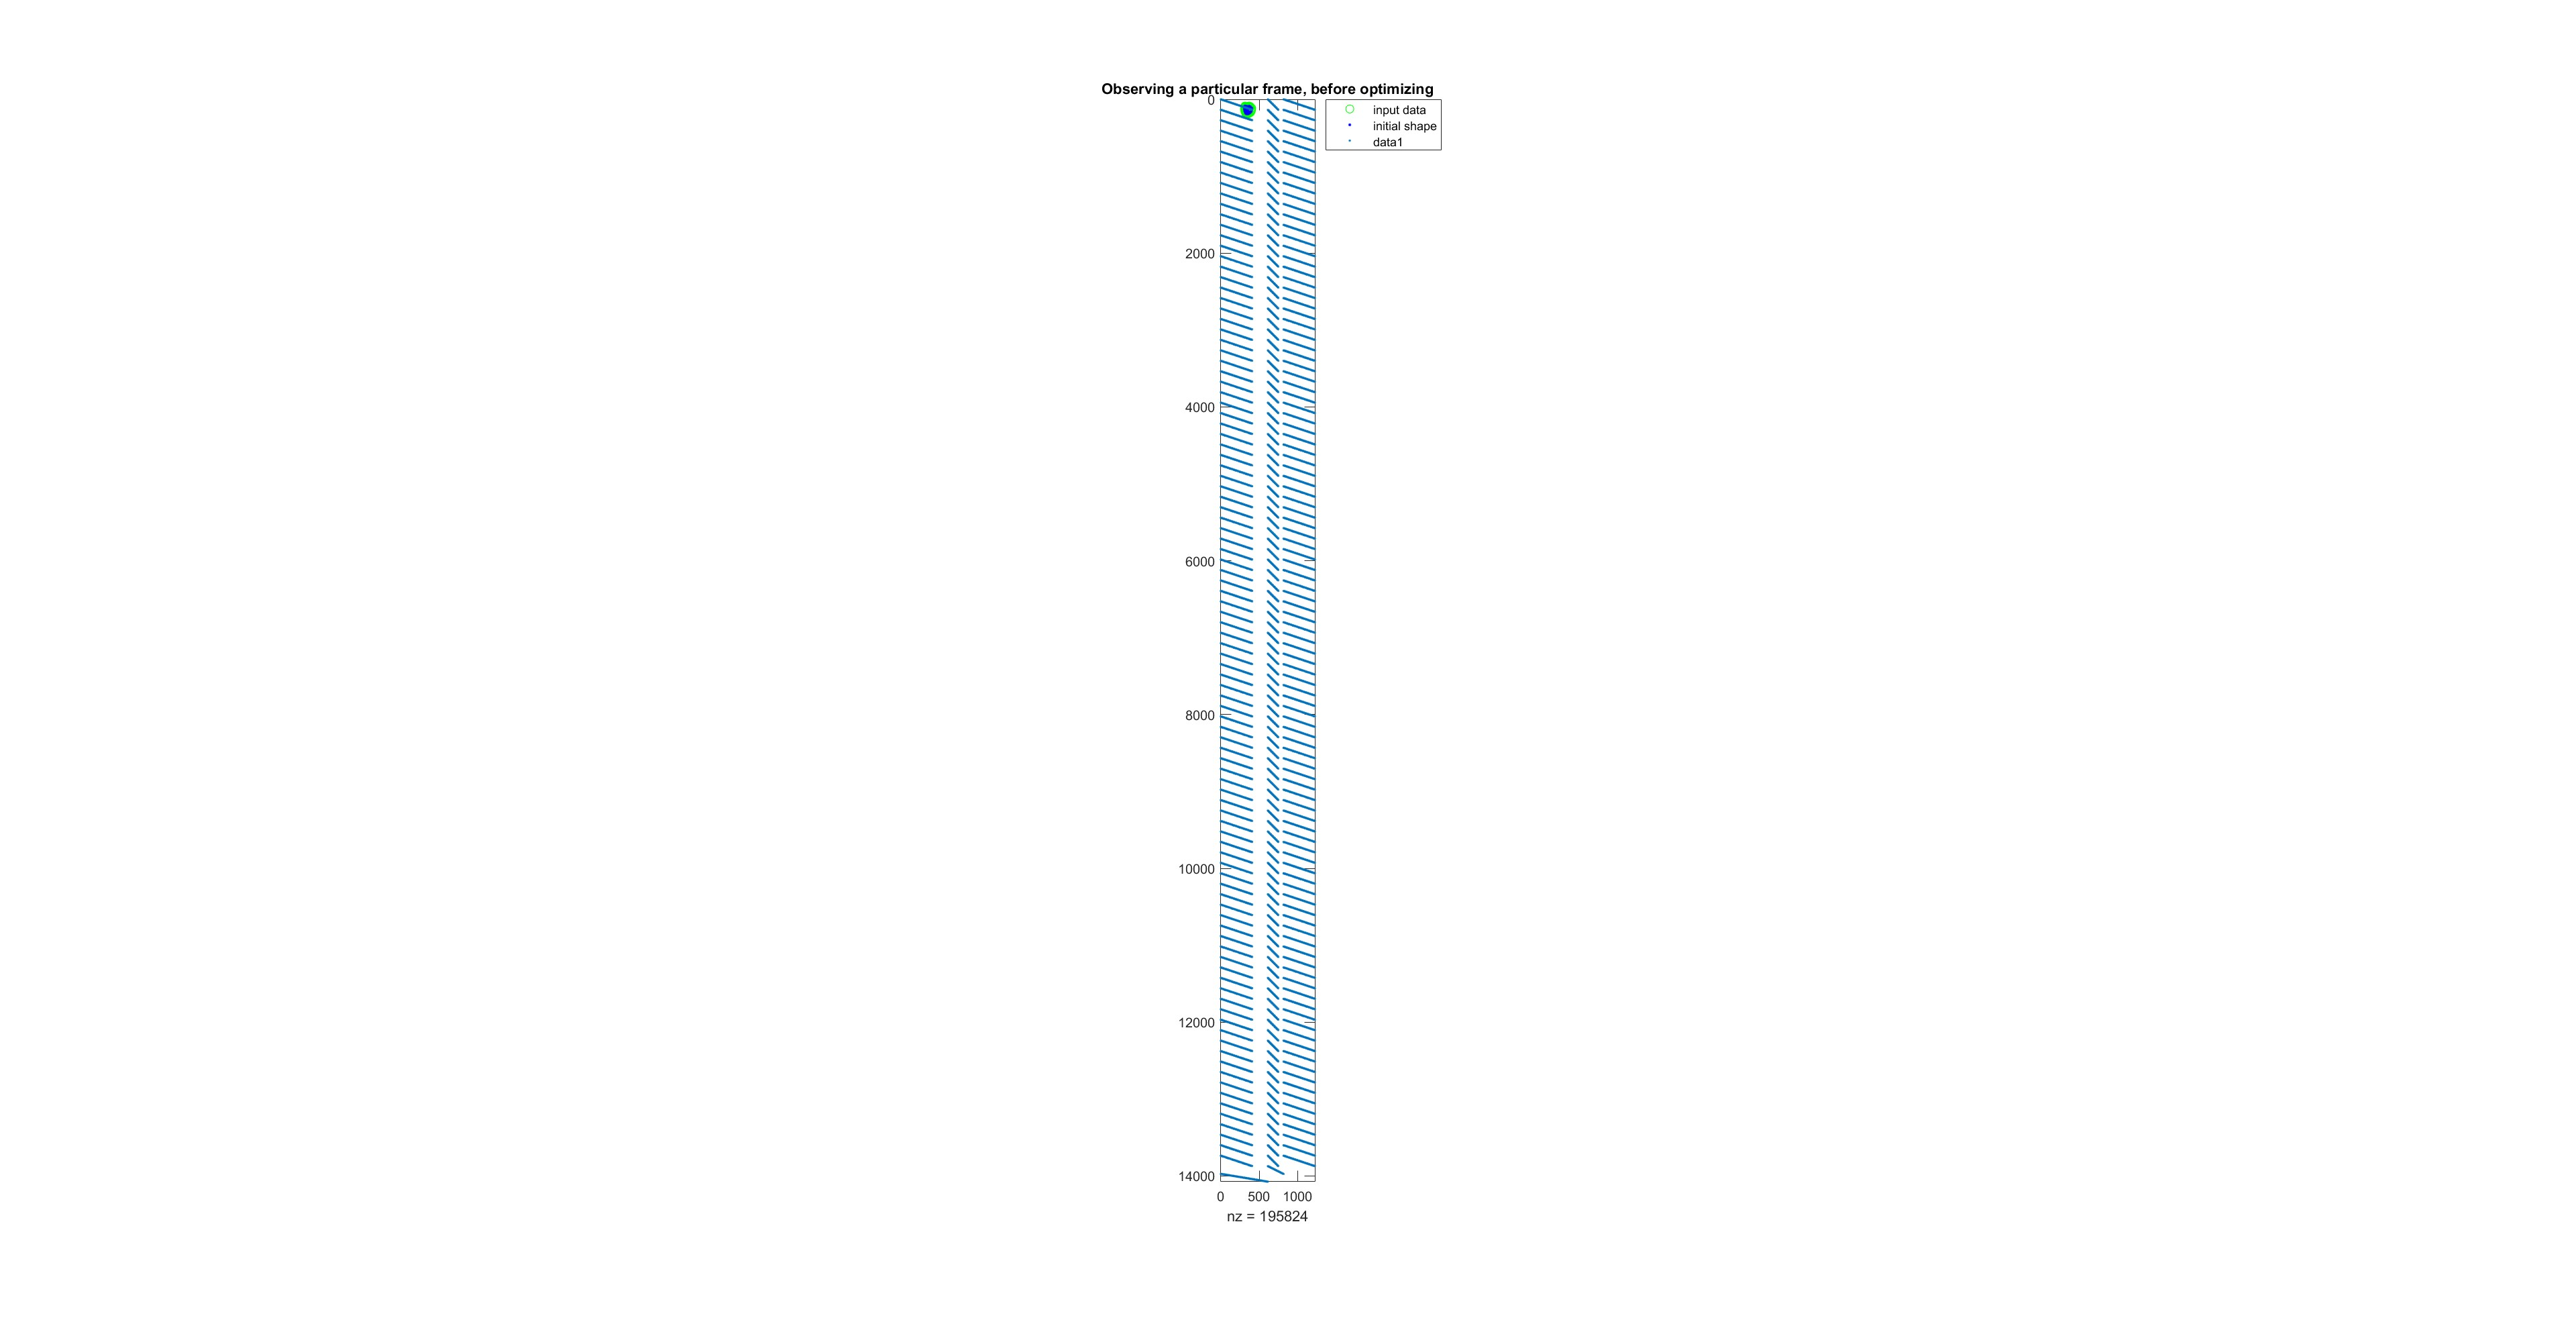
\includegraphics[width=1.0\textwidth]{T2/J}
    \caption{Jacobian result}
    \label{fig:J}
\end{figure}
\newpage
\subsection{Examples:}
\noindent Here we will show how to reconstruct the human face with the given frames and using the following input parameters:

\begin{itemize}
\item low-rank $K$(it is the number of bases): $2$
\item camera\_prior (it means that the $R$ prior is active): $1$
\item coeff\_prior (it means that the $L$ prior is active): $1$
\item number of optimizer iterations: $50$
\end{itemize}
\noindent In Figure \ref{fig:coodinates2D} we can see the comparison of the input points of a frame in green against the estimated points of that frame in blue color.\\

\begin{figure}[h!]
    \centering
    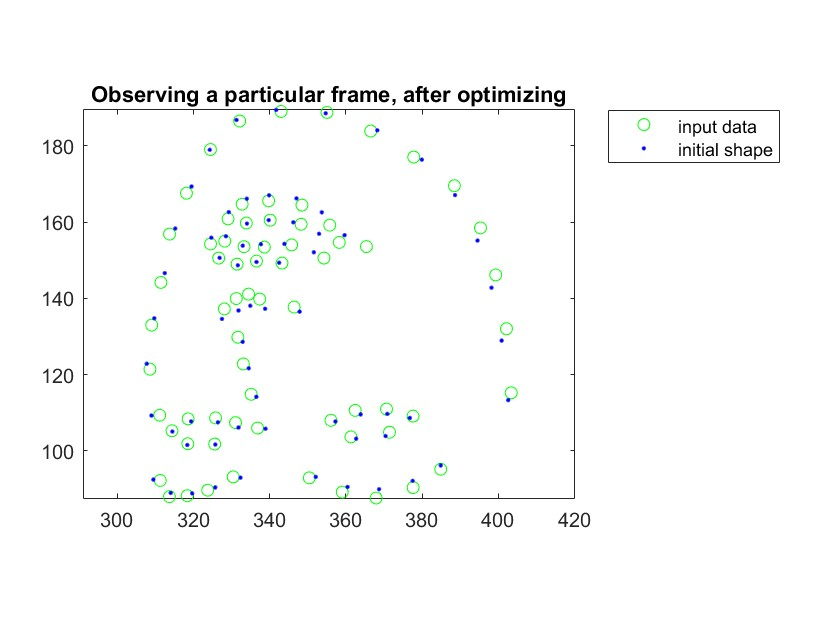
\includegraphics[scale=0.37]{T2/coodinates2D}
    \caption{Input points compared to optimized points}
    \label{fig:coodinates2D}
\end{figure}

\noindent In Figure \ref{fig:coordinates3D} we can see the estimated 3D points for a frame.\\ 
\begin{figure}[h!]
    \centering
    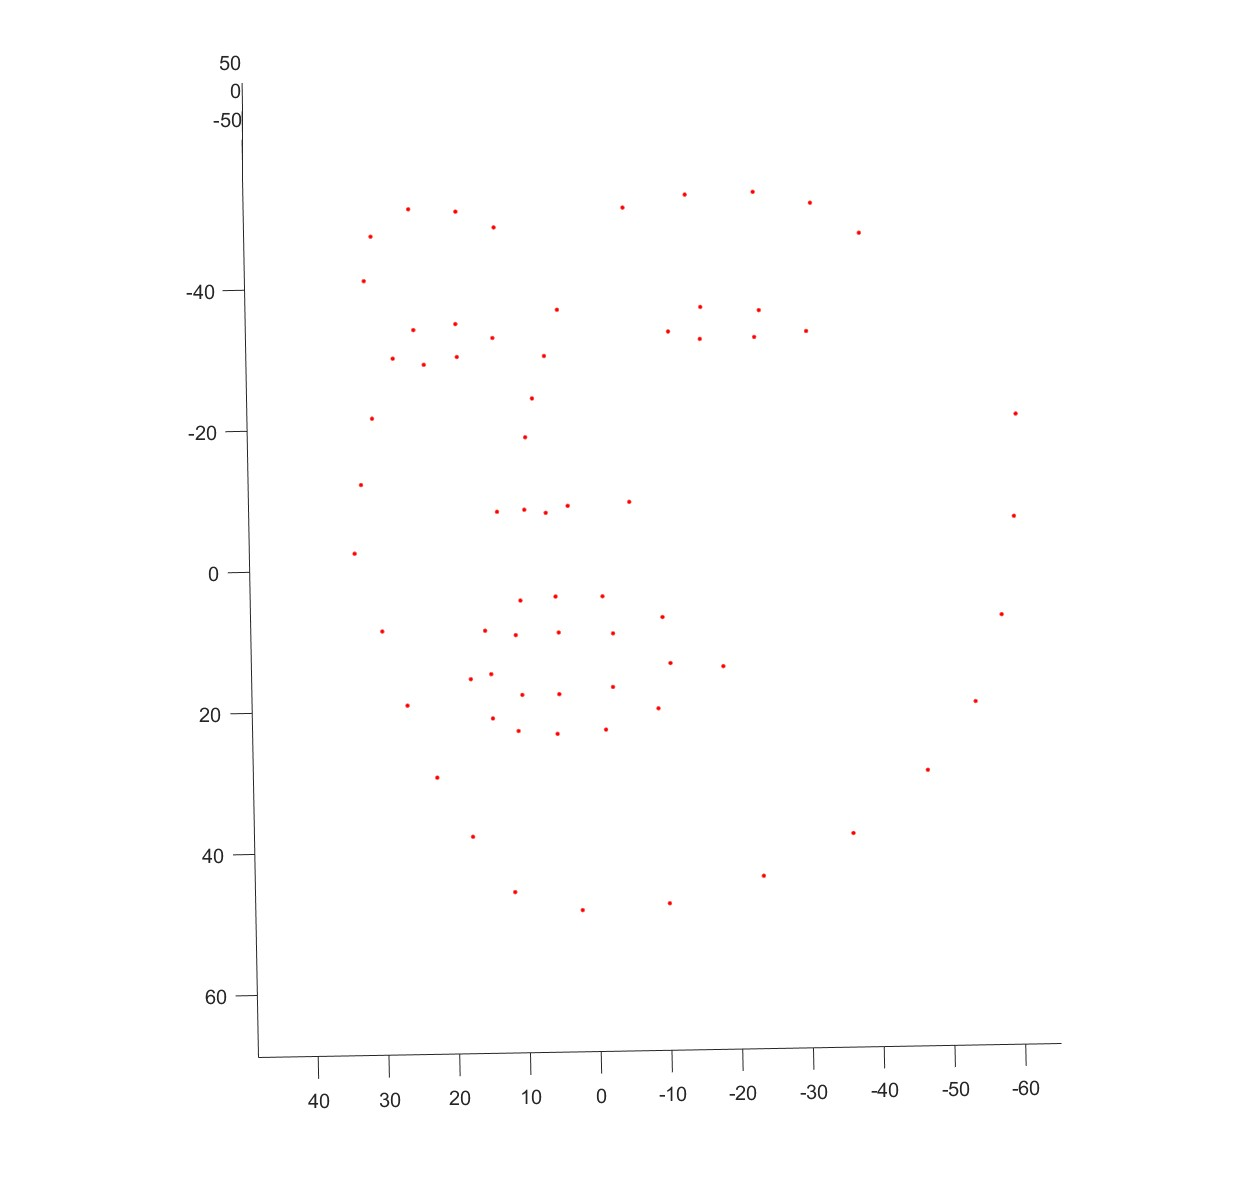
\includegraphics[scale=0.25]{T2/coordinates3D}
    \caption{3D reconstruction}
    \label{fig:coordinates3D}
\end{figure}

\noindent In Figure \ref{fig:steps} we see the calculation of each of the 50 optimizations, this method has a high cost in performance, but a good result is achieved as shown by the low error at the end.\\
\begin{figure}[h!]
    \centering
    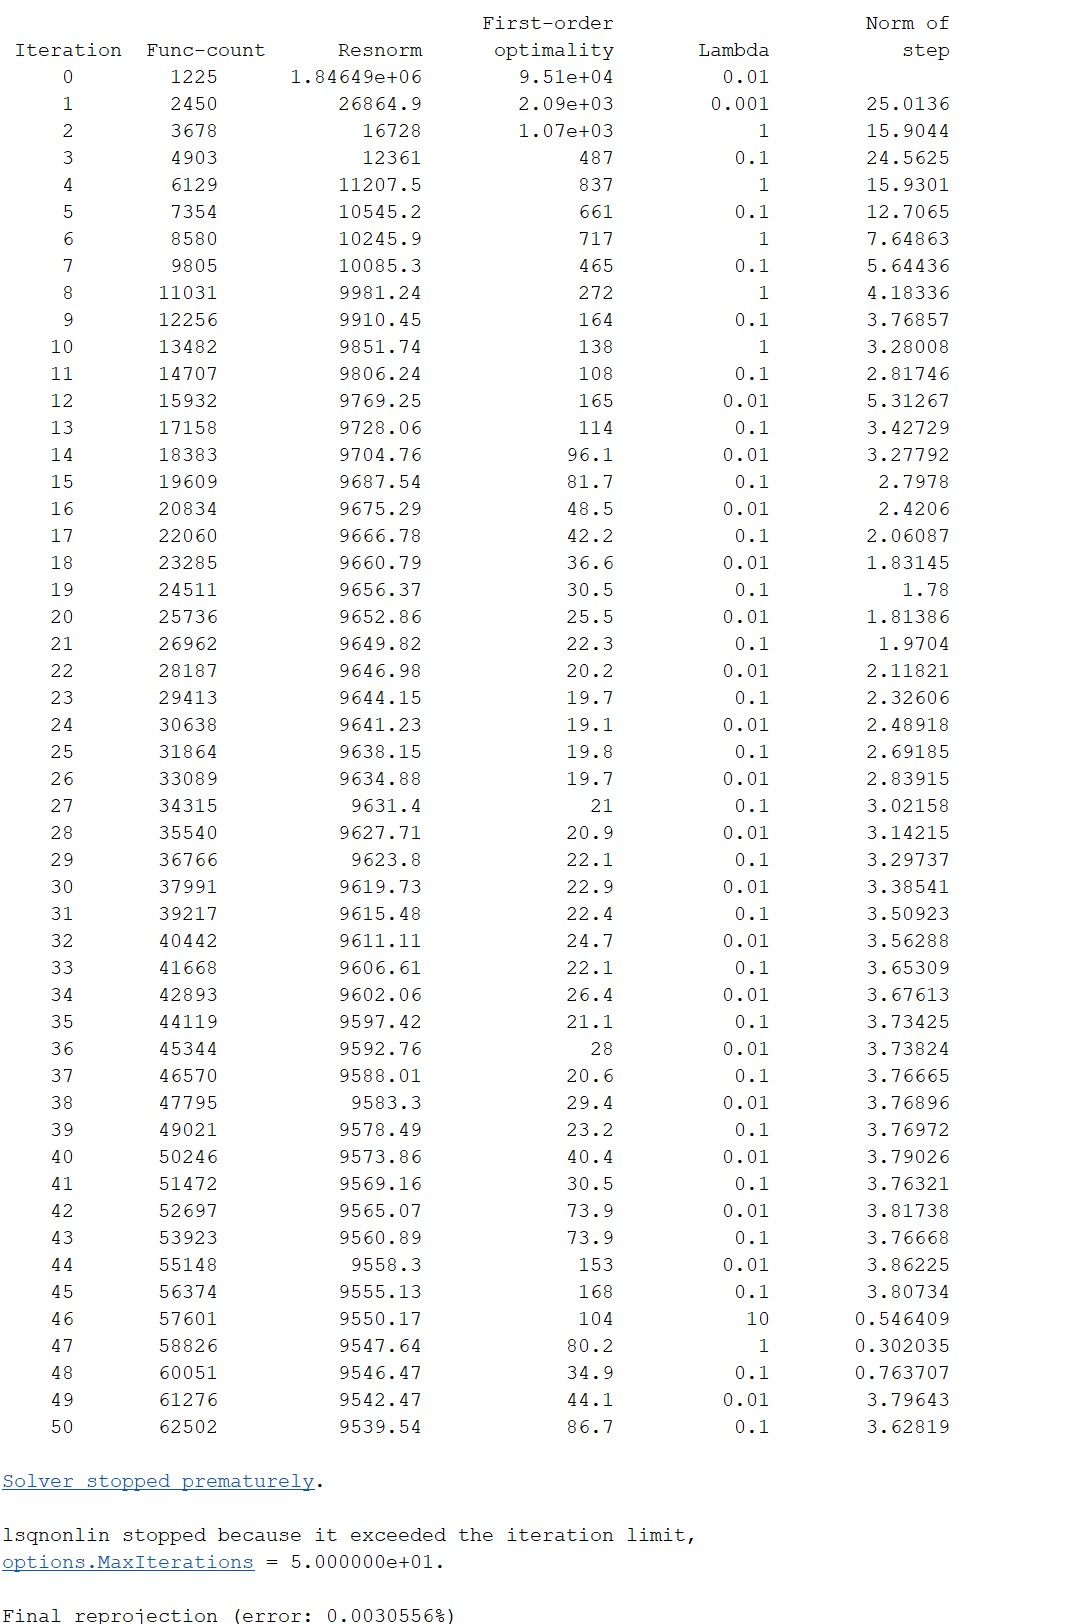
\includegraphics[scale=0.69]{T2/steps}
    \caption{Optimizer iterations}
    \label{fig:steps}
\end{figure}

\noindent For this model, if we increase the rank of the shape basis $k$, the approximation can improve, but also the performance cost increases. On the other hand, the factorization method, assuming a low-rank trajectory model, has a lower performance cost than the non-linear optimization method, assuming a low-rank shape model. 

